\documentclass{beamer}
% Class options include: notes, notesonly, handout, trans,
%                        hidesubsections, shadesubsections,
%                        inrow, blue, red, grey, brown

% Theme for beamer presentation.
\usepackage{beamerthemesplit} 
% Other themes include: beamerthemebars, beamerthemelined, 
%                       beamerthemetree, beamerthemetreebars  

\title[Commitment Institutions and Instability]{Commitment Institutions and Electoral and Political Instability}
\subtitle{A Reduced-Form Approach}
\author{Isaac Liu}
\date{\today}

\usepackage{graphicx} % http://ctan.org/pkg/graphicx
\usepackage{amsmath}
\usepackage{geometry}
\usepackage{amsfonts}
\usepackage[english]{babel}
\usepackage{amssymb}
\usepackage{graphicx}
\usepackage{float}
\usepackage{hyperref}
\usepackage{multirow}
\usepackage{pdflscape}
\usepackage{caption}
\usepackage{pdflscape}
\usepackage{outlines}
\usepackage{subcaption}

\usepackage{framed}

\usepackage{tabularx, booktabs}

\usepackage{standalone}

\usepackage[autostyle, english = american]{csquotes}
\MakeOuterQuote{"}

\usepackage{comment}

\hypersetup{
    colorlinks=true,
    linkcolor=white,
    filecolor=black,      
    urlcolor=black,
}

\setbeamertemplate{navigation symbols}{}

\begin{document}

    \begin{frame}
        \titlepage
    \end{frame}

    \begin{frame}
        \frametitle{\small Do the commitment institutions of central bank independence and fixed exchange rates affect electoral and political instability?}
        \begin{itemize}
            \item Potential theories:
            \begin{itemize}
                \item Net Welfare Benefits
                \begin{itemize}
                    \item Inflation time inconsistency problem solved
                    \item Increased political efficacy, access to capital
                    \item Economic voting theory thus implies increased stability
                \end{itemize}
                \item Political Business Cycles
                \begin{itemize}
                    \item Inability to manipulate economy or satisfy partisans
                    \item Monetary (perhaps fiscal) policy limited
                    \item Economic voting theory thus implies decreased stability
                \end{itemize}
            \end{itemize}
        \end{itemize}

        \begin{figure}[h]
    
            \begin{subfigure}[h]{0.475\textwidth}
                \centering
                
\includegraphics[width=0.95\hsize]{../../Output/Figures/Fire_JP_Headline.png} 
            \end{subfigure}
            \hfill
            \begin{subfigure}[h]{0.475\textwidth}
                \centering
                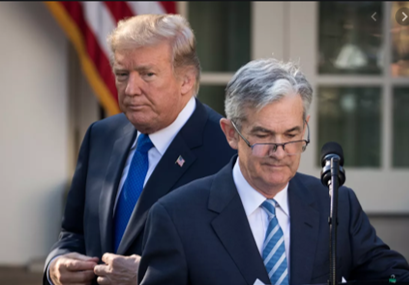
\includegraphics[width=0.95\hsize]{../../Output/Figures/Trump_and_JP.png}
            \end{subfigure}
    
        \end{figure}

    \end{frame}

    \begin{frame}
        \frametitle{Theoretical Mechanisms}
        \begin{figure}[h!]
            \centering
            \caption{Effects of Limiting Institutions on Instability}
                \begin{subfigure}{.5\textwidth}
                    \centering
                    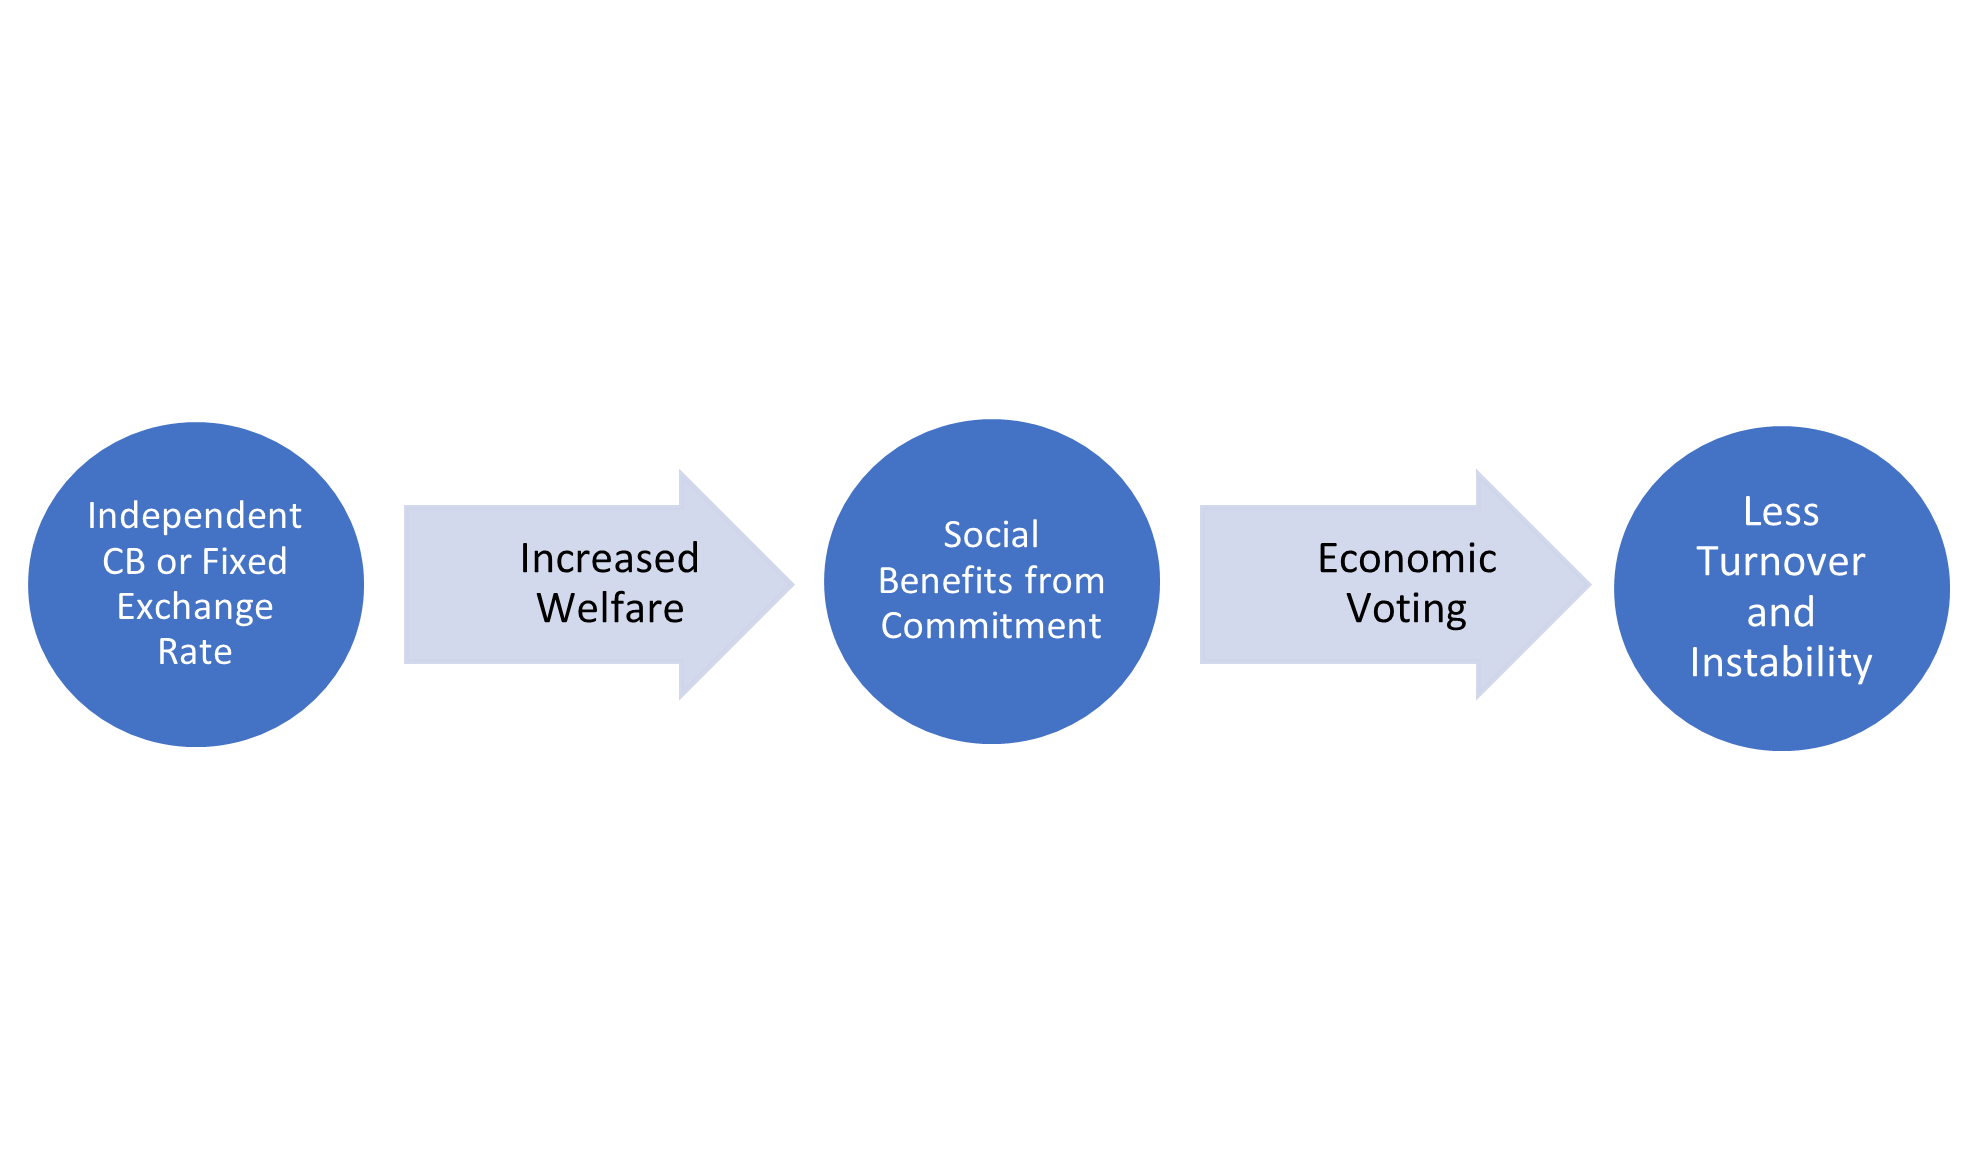
\includegraphics[width=\linewidth,keepaspectratio=true]{../../Output/Figures/Social_Welfare_Model.png}
                    \caption{Welfare Model}
                \end{subfigure}%
                \begin{subfigure}{.5\textwidth}
                    \centering
                    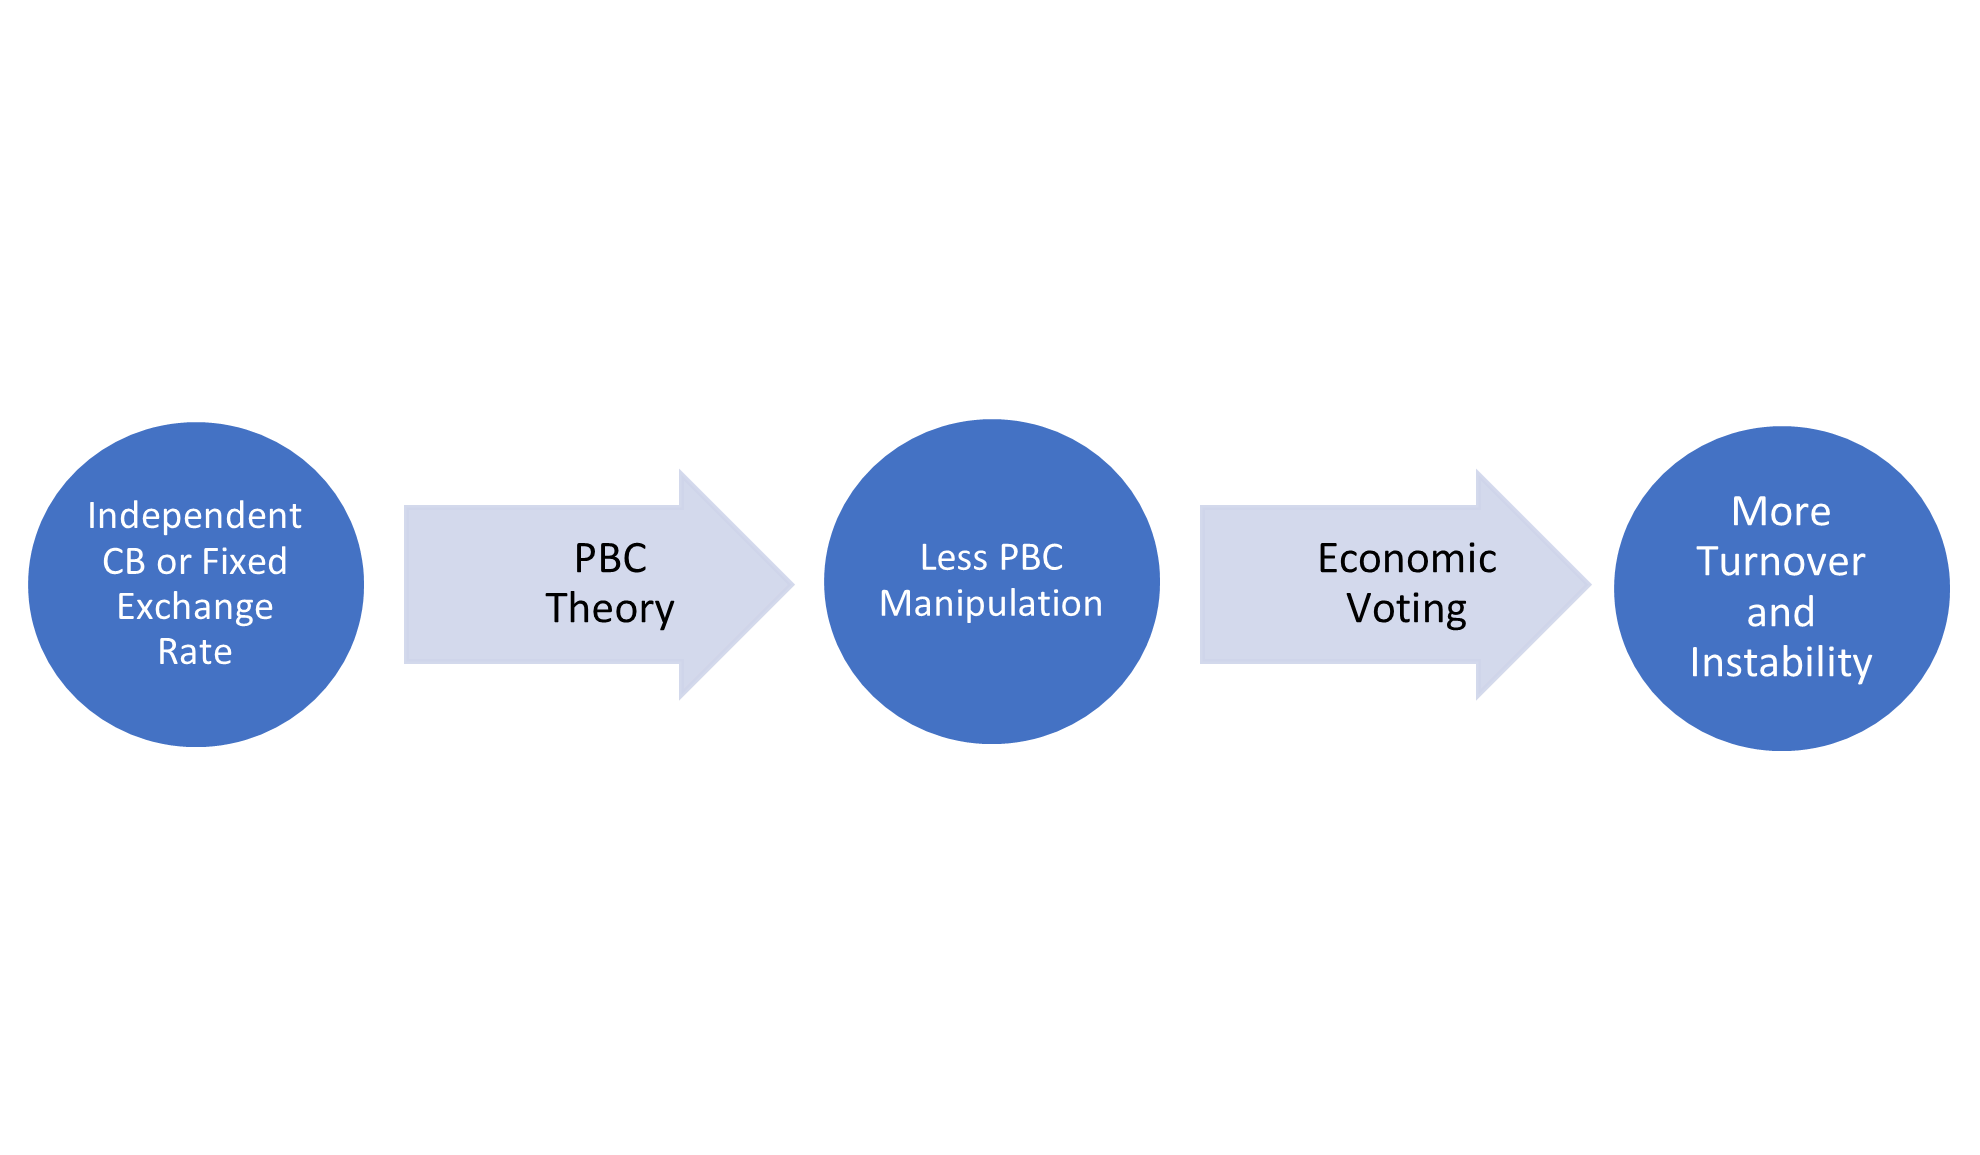
\includegraphics[width=\linewidth,keepaspectratio=true]{../../Output/Figures/Political_Business_Cycle_Model.png}
                    \caption{Political Business Cycle Model}
                \end{subfigure}
        \end{figure}
    \end{frame}

    \begin{frame}
        \frametitle{Literature}
        \begin{itemize}
            \item Bernhard and Leblang (2002)
            \begin{itemize}
                \item OLS, 16 parliamentary democracies since 1970s
                \item CBI increases cabinet duration by 3 months, fixed rates by 5 months, especially with open trade and capital account
            \end{itemize}
            \item Clark, Golder, and Poast (2013)
            \begin{itemize}
                \item Survival analysis, 19 OECD countries since 1970s
                \item Both institutions increase leader survival but only after 7 years in office
            \end{itemize}
            \item Contribution:
            \begin{itemize}
                \item Far larger dataset including non/semi-democracies
                \item More consideration of endogeneity: choice of institutions based on stability consideration, de jure/de facto independence difference
                \item Political, not just electoral stability (coups, civil wars, etc), consideration for specific governmental positions
            \end{itemize}
        \end{itemize}
    \end{frame}

    \begin{frame}
        \frametitle{Data}
        \begin{itemize}
            \item Panel of 192 countries, 1970-2016
            \item Varieties of Democracy
            \begin{itemize}
                \item Turnover variables: v2eltturnhog (Head of Government, HOG), v2elturnhos (Head of State, HOG), v2eltvrig (Lower House, L.H.)
                \item 0 for same individual (no turnover), 1 for same party or coalition (half turnover), 2 for new party and individual (full turnover)
                \item WGI Political Violence (positive value implies more stable)
                \item Instability Event- coup, civil war, internal conflict indicator
            \end{itemize}
            \item Garriga (Cukierman, Webb, Neyapti)- de jure CBI
            \item Dreher et al.- Irregular turnover of governor- de facto CBI
            \item Reinhart, Rogoff Exchange Rates: 16 categories (higher implies closer to a pure float)
        \end{itemize}
    \end{frame}

    \begin{frame}
        \frametitle{Results}
        \begin{itemize}
            \item Separate regressions for de jure and de facto CBI (bad control problem)
            \item FEs, clustered SEs
            \item De jure CBI and more instability: political business cycles
            \item De facto CBI (high irregular turnover) and less lower chamber turnover
            \item Fixed rate and less HOS turnover
            \item De facto CBI, fixed rates and less instability: welfare benefits?
        \end{itemize}
    \end{frame}

    \begin{frame}
        \frametitle{Fixed Effects Regression with Clustered Standard Errors}
        {
            \let\oldcentering\centering
            \renewcommand\centering{\tiny\oldcentering}
            {
\def\sym#1{\ifmmode^{#1}\else\(^{#1}\)\fi}
\begin{tabular}{l*{5}{c}}
\hline\hline
                &\multicolumn{1}{c}{(1)}&\multicolumn{1}{c}{(2)}&\multicolumn{1}{c}{(3)}&\multicolumn{1}{c}{(4)}&\multicolumn{1}{c}{(5)}\\
                &\multicolumn{1}{c}{Head of Govt. Turnover}&\multicolumn{1}{c}{Head of State Turnover}&\multicolumn{1}{c}{Lower House Turnover}&\multicolumn{1}{c}{WB Political Stability (Absence of Violence)}&\multicolumn{1}{c}{Instability Event Indicator}\\
\hline
De Jure CBI (CNW Index)&    0.276         &    0.303\sym{*}  &    0.389\sym{*}  &   -0.417\sym{**} &    1.000\sym{***}\\
                &   (1.44)         &   (2.30)         &   (1.99)         &  (-2.75)         &  (11.15)         \\
[1em]
Exchange Rate Classification (RR inverted, higher = more fixed)&  -0.0120         &  -0.0207\sym{***}& -0.00615         &   0.0106         &  0.00690         \\
                &  (-1.61)         &  (-3.45)         &  (-0.71)         &   (1.69)         &   (1.33)         \\
[1em]
Constant        &    0.618\sym{***}&    0.390\sym{***}&    0.535\sym{***}&   0.0283         &   -0.113\sym{*}  \\
                &   (6.15)         &   (5.43)         &   (4.99)         &   (0.31)         &  (-2.20)         \\
\hline
Observations    &     1399         &     1399         &     1141         &     2141         &     4207         \\
\hline\hline
\multicolumn{6}{l}{\footnotesize \textit{t} statistics in parentheses}\\
\multicolumn{6}{l}{\footnotesize \sym{*} \(p<0.05\), \sym{**} \(p<0.01\), \sym{***} \(p<0.001\)}\\
\end{tabular}
}

        }
    \end{frame}

    \begin{frame}
        \frametitle{Fixed Effects Regression with Clustered Standard Errors}
        {
            \let\oldcentering\centering
            \renewcommand\centering{\tiny\oldcentering}
            \begin{table}[htbp]\centering
\def\sym#1{\ifmmode^{#1}\else\(^{#1}\)\fi}
\caption{De Facto CBI, Fixed Effects Regression with Clustered Standard Errors \label{multIndFEDF}}
\begin{tabular}{l*{5}{c}}
\hline\hline
                    &\multicolumn{1}{c}{(1)}&\multicolumn{1}{c}{(2)}&\multicolumn{1}{c}{(3)}&\multicolumn{1}{c}{(4)}&\multicolumn{1}{c}{(5)}\\
                    &\multicolumn{1}{c}{Head of Govt. Turnover}&\multicolumn{1}{c}{Head of State Turnover}&\multicolumn{1}{c}{Lower House Turnover}&\multicolumn{1}{c}{WB Political Stability (Absence of Violence)}&\multicolumn{1}{c}{Instability Event Indicator}\\
\hline
(Lack of) Irregular &      -0.117         &     -0.0512         &      -0.211\sym{**} &     0.00955         &      0.0244         \\
CB Governor Turnover (higher = more de facto CBI)&     (-1.68)         &     (-0.81)         &     (-2.81)         &      (0.36)         &      (1.36)         \\
[1em]
Exchange Rate       &    -0.00548         &     -0.0117\sym{*}  &     0.00444         &      0.0153\sym{*}  &      0.0128\sym{**} \\
Classification (RR inverted, higher = more fixed)&     (-0.82)         &     (-2.06)         &      (0.53)         &      (2.08)         &      (2.73)         \\
[1em]
Constant            &       0.805\sym{***}&       0.521\sym{***}&       0.865\sym{***}&      -0.247\sym{***}&       0.261\sym{***}\\
                    &      (9.91)         &      (7.75)         &      (9.43)         &     (-3.54)         &      (6.77)         \\
\hline
Observations        &        1651         &        1651         &        1334         &        2669         &        4491         \\
\hline\hline
\multicolumn{6}{l}{\footnotesize \textit{t} statistics in parentheses}\\
\multicolumn{6}{l}{\footnotesize \sym{*} \(p<0.05\), \sym{**} \(p<0.01\), \sym{***} \(p<0.001\)}\\
\end{tabular}
\end{table}

        }
    \end{frame}

    \begin{frame}
        \frametitle{Ordered Logit (Mean Marginal Effects)}
        \begin{itemize}
            \item Nothing changes in terms of significance, except for fixed rates and HOG
            \item xtologit; random effects
        \end{itemize}
    \end{frame}

    \begin{frame}
        \frametitle{Ordered Logit Mean Marginal Effects}
        {
            \let\oldcentering\centering
            \renewcommand\centering{\tiny\oldcentering}
            {
\def\sym#1{\ifmmode^{#1}\else\(^{#1}\)\fi}
\begin{tabular*}{\linewidth}{@{\hskip\tabcolsep\extracolsep\fill}l*{3}{c}}
\hline\hline
                &\multicolumn{1}{c}{(1)}&\multicolumn{1}{c}{(2)}&\multicolumn{1}{c}{(3)}\\
                &\multicolumn{1}{c}{}&\multicolumn{1}{c}{}&\multicolumn{1}{c}{}\\
\hline
De Jure CBI (CNW Index)&                  &                  &                  \\
1.\_predict      &   -0.146         &   -0.208\sym{***}&   -0.316\sym{***}\\
                &  (-1.93)         &  (-3.54)         &  (-3.65)         \\
[1em]
2.\_predict      &   0.0152         &   0.0390\sym{***}&   0.0980\sym{**} \\
                &   (1.80)         &   (3.32)         &   (3.21)         \\
[1em]
3.\_predict      &    0.131         &    0.169\sym{***}&    0.218\sym{***}\\
                &   (1.93)         &   (3.47)         &   (3.68)         \\
\hline
Exchange Rate Classification (RR inverted, higher = more fixed)&                  &                  &                  \\
1.\_predict      &  0.00792\sym{*}  &  0.00896\sym{**} &  0.00392         \\
                &   (2.45)         &   (3.21)         &   (0.96)         \\
[1em]
2.\_predict      &-0.000826\sym{*}  & -0.00168\sym{**} & -0.00122         \\
                &  (-2.22)         &  (-3.00)         &  (-0.96)         \\
[1em]
3.\_predict      & -0.00710\sym{*}  & -0.00728\sym{**} & -0.00271         \\
                &  (-2.46)         &  (-3.18)         &  (-0.96)         \\
\hline
Observations    &     1399         &     1399         &     1141         \\
\hline\hline
\multicolumn{4}{l}{\footnotesize \textit{t} statistics in parentheses}\\
\multicolumn{4}{l}{\footnotesize \sym{*} \(p<0.05\), \sym{**} \(p<0.01\), \sym{***} \(p<0.001\)}\\
\end{tabular*}
}

        }
    \end{frame}

    \begin{frame}
        \frametitle{Ordered Logit Mean Marginal Effects}
        {
            \let\oldcentering\centering
            \renewcommand\centering{\tiny\oldcentering}
            \begin{table}[htbp]\centering
\def\sym#1{\ifmmode^{#1}\else\(^{#1}\)\fi}
\caption{De Facto CBI, Mean Marginal Effects, Ordered Logit Panel Regression, Random Effects, Clustered Standard Errors \label{ordLogDF}}
\begin{tabular}{l*{3}{c}}
\toprule
                                        &\multicolumn{1}{c}{(1)}&\multicolumn{1}{c}{(2)}&\multicolumn{1}{c}{(3)}\\
                                        &\multicolumn{1}{c}{}&\multicolumn{1}{c}{}&\multicolumn{1}{c}{}\\
\midrule
(Lack of) Irregular CB Governor Turnover (higher = more de facto CBI)&                  &                  &                  \\
1.\_predict                              &   0.0734\sym{*}  &   0.0356         &    0.119\sym{**} \\
                                        &   (2.23)         &   (1.30)         &   (3.19)         \\
\addlinespace
2.\_predict                              & -0.00756\sym{*}  & -0.00655         &  -0.0296\sym{**} \\
                                        &  (-2.02)         &  (-1.24)         &  (-3.05)         \\
\addlinespace
3.\_predict                              &  -0.0658\sym{*}  &  -0.0290         &  -0.0890\sym{**} \\
                                        &  (-2.23)         &  (-1.31)         &  (-3.14)         \\
\midrule
Exchange Rate Classification (RR inverted, higher = more fixed)&                  &                  &                  \\
1.\_predict                              &  0.00384         &  0.00473         & -0.00440         \\
                                        &   (1.32)         &   (1.93)         &  (-1.19)         \\
\addlinespace
2.\_predict                              &-0.000396         &-0.000870         &  0.00110         \\
                                        &  (-1.27)         &  (-1.87)         &   (1.18)         \\
\addlinespace
3.\_predict                              & -0.00345         & -0.00386         &  0.00331         \\
                                        &  (-1.32)         &  (-1.92)         &   (1.19)         \\
\midrule
Observations                            &     1651         &     1651         &     1334         \\
\bottomrule
\multicolumn{4}{l}{\footnotesize \textit{t} statistics in parentheses}\\
\multicolumn{4}{l}{\footnotesize \sym{*} \(p<0.05\), \sym{**} \(p<0.01\), \sym{***} \(p<0.001\)}\\
\end{tabular}
\end{table}

        }
    \end{frame}

    \begin{frame}
        \frametitle{Panel Logit (Binary Instability Event Variable) Mean Marginal Effects}
        \begin{itemize}
            \item Fixed effects
            \item More evidence that de jure CBI increases political instability
            \item Fixed exchange rate (low RR rate classification) increases political instability, but very small effect size
        \end{itemize}
    \end{frame}

    \begin{frame}
        \frametitle{Binary Instability Event Logit, Mean Marginal Effects}
        {
            \let\oldcentering\centering
            \renewcommand\centering{\tiny\oldcentering}
            \begin{table}[htbp]\centering
\def\sym#1{\ifmmode^{#1}\else\(^{#1}\)\fi}
\caption{De Jure CBI, Instability Event Panel Logit, Fixed Effects and Clustered Standard Errors, Mean Marginal Effects \label{margsJustBinInstabEventDJ}}
\begin{tabular}{l*{1}{c}}
\toprule
                                        &\multicolumn{1}{c}{(1)}\\
                                        &\multicolumn{1}{c}{}\\
\midrule
De Jure CBI (CNW Index)                 &     0.376\sym{***}\\
                                        &   (12.93)         \\
\addlinespace
Exchange Rate Classification (RR        &   0.00227\sym{**} \\
inverted, higher = more fixed)          &    (2.99)         \\
\midrule
Observations                            &      3912         \\
\bottomrule
\multicolumn{2}{l}{\footnotesize \textit{t} statistics in parentheses}\\
\multicolumn{2}{l}{\footnotesize \sym{*} \(p<0.05\), \sym{**} \(p<0.01\), \sym{***} \(p<0.001\)}\\
\end{tabular}
\end{table}

        }
    \end{frame}

    \begin{frame}
        \frametitle{Binary Instability Event Logit, Mean Marginal Effects}
        {
            \let\oldcentering\centering
            \renewcommand\centering{\tiny\oldcentering}
            \begin{table}[htbp]\centering
\def\sym#1{\ifmmode^{#1}\else\(^{#1}\)\fi}
\caption{Instability Event Panel Logit, Fixed Effects and Clustered Standard Errors, Mean Marginal Effects \label{margsJustBinInstabEventDF}}
\begin{tabular}{l*{1}{c}}
\toprule
                                        &\multicolumn{1}{c}{(1)}\\
                                        &\multicolumn{1}{c}{}\\
\midrule
De facto CBI                            &   0.0282         \\
                                        &   (1.18)         \\
\addlinespace
Fixed Rate                              &   0.0152\sym{***}\\
                                        &   (6.71)         \\
\midrule
Observations                            &     4163         \\
\bottomrule
\multicolumn{2}{l}{\footnotesize \textit{t} statistics in parentheses}\\
\multicolumn{2}{l}{\footnotesize \sym{*} \(p<0.05\), \sym{**} \(p<0.01\), \sym{***} \(p<0.001\)}\\
\end{tabular}
\end{table}

        }
    \end{frame}

    \begin{frame}
        \frametitle{IV1: Tertiary Ed Enrollment (CBI), Aggregate GDP (Fixed Rate)}
        \begin{itemize}
            \item Good first stages
            \item Poor exclusion restrictions for political stability, better ones for electoral stability/turnover
            \item De jure CBI now increases lower chamber turnover, but no longer HOS
            \item Fixed rates appear to increase lower chamber turnover
            \item De facto CBI more or less insignificant
        \end{itemize}
    \end{frame}

    \begin{frame}
        \frametitle{Tertiary Education and Aggregate GDP Instruments}
        {
            \let\oldcentering\centering
            \renewcommand\centering{\tiny\oldcentering}
            {
\def\sym#1{\ifmmode^{#1}\else\(^{#1}\)\fi}
\begin{tabular*}{\linewidth}{@{\hskip\tabcolsep\extracolsep\fill}l*{5}{c}}
\toprule
                &\multicolumn{1}{c}{(1)}&\multicolumn{1}{c}{(2)}&\multicolumn{1}{c}{(3)}&\multicolumn{1}{c}{(4)}&\multicolumn{1}{c}{(5)}\\
                &\multicolumn{1}{c}{Head of Govt. Turnover}&\multicolumn{1}{c}{Head of State Turnover}&\multicolumn{1}{c}{Lower House Turnover}&\multicolumn{1}{c}{WB Political Stability (Absence of Violence)}&\multicolumn{1}{c}{Instability Event Indicator}\\
\midrule
De Jure CBI (CNW Index)&    0.629         &   -0.478         &    0.847\sym{*}  &    6.976\sym{***}&    0.835\sym{***}\\
                &   (1.55)         &  (-1.42)         &   (1.97)         &  (13.27)         &   (4.30)         \\
\addlinespace
Exchange Rate Classification (RR inverted, higher = more fixed)& -0.00669         &   0.0171         &   0.0266         &  -0.0865\sym{**} &  -0.0295         \\
                &  (-0.19)         &   (0.51)         &   (0.76)         &  (-2.84)         &  (-1.66)         \\
\addlinespace
Constant        &    0.401         &    0.576\sym{*}  &   0.0636         &   -3.422\sym{***}&    0.292         \\
                &   (1.28)         &   (2.01)         &   (0.22)         &  (-9.22)         &   (1.65)         \\
\midrule
Observations    &      851         &      851         &      686         &     1865         &     2047         \\
\bottomrule
\multicolumn{6}{l}{\footnotesize \textit{t} statistics in parentheses}\\
\multicolumn{6}{l}{\footnotesize \sym{*} \(p<0.05\), \sym{**} \(p<0.01\), \sym{***} \(p<0.001\)}\\
\end{tabular*}
}

        }
    \end{frame}

    \begin{frame}
        \frametitle{Tertiary Education and Aggregate GDP Instruments}
        {
            \let\oldcentering\centering
            \renewcommand\centering{\tiny\oldcentering}
            {
\def\sym#1{\ifmmode^{#1}\else\(^{#1}\)\fi}
\begin{tabular}{l*{5}{c}}
\hline\hline
                    &\multicolumn{1}{c}{(1)}&\multicolumn{1}{c}{(2)}&\multicolumn{1}{c}{(3)}&\multicolumn{1}{c}{(4)}&\multicolumn{1}{c}{(5)}\\
                    &\multicolumn{1}{c}{Head of Govt. Turnover}&\multicolumn{1}{c}{Head of State Turnover}&\multicolumn{1}{c}{Lower House Turnover}&\multicolumn{1}{c}{WB Political Stability (Absence of Violence)}&\multicolumn{1}{c}{Instability Event Indicator}\\
\hline
(Lack of) Irregular &       1.295         &      -0.626         &       2.071         &       39.47\sym{*}  &      -18.01         \\
CB Governor Turnover (higher = more de facto CBI)&      (1.19)         &     (-0.74)         &      (1.66)         &      (1.97)         &     (-0.46)         \\
[1em]
Exchange Rate       &      0.0152         &     -0.0101         &      0.0864\sym{*}  &       0.581         &      -0.131         \\
Classification (RR inverted, higher = more fixed)&      (0.46)         &     (-0.32)         &      (2.08)         &      (1.49)         &     (-0.47)         \\
[1em]
Constant            &      -0.538         &       1.085         &      -1.708         &      -40.72         &       17.29         \\
                    &     (-0.50)         &      (1.32)         &     (-1.39)         &     (-1.96)         &      (0.48)         \\
\hline
Observations        &         962         &         962         &         788         &        2236         &        2011         \\
\hline\hline
\multicolumn{6}{l}{\footnotesize \textit{t} statistics in parentheses}\\
\multicolumn{6}{l}{\footnotesize \sym{*} \(p<0.05\), \sym{**} \(p<0.01\), \sym{***} \(p<0.001\)}\\
\end{tabular}
}

        }
    \end{frame}

    \begin{frame}
        \frametitle{IV2: Population Share Social Science/Business Grads (CBI), Aggregate GDP (Fixed Rates)}
        \begin{itemize}
            \item Better exclusion restriction
            \item Very limited data but strong result for de jure CBI and political instability
            \item Fixed rates again associated with lower house turnover in the de facto specification
        \end{itemize}
    \end{frame}

    \begin{frame}
        \frametitle{Population Share Social Science/Business Grads and Agg GDP Instruments}
        {
            \let\oldcentering\centering
            \renewcommand\centering{\tiny\oldcentering}
            \begin{table}[htbp]\centering
\def\sym#1{\ifmmode^{#1}\else\(^{#1}\)\fi}
\caption{Instruments of Social Science/Business Graduates Population Share and Aggregate GDP, Robust Standard Errors \label{ifivs3}}
\begin{tabular}{l*{5}{c}}
\toprule
                                        &\multicolumn{1}{c}{(1)}&\multicolumn{1}{c}{(2)}&\multicolumn{1}{c}{(3)}&\multicolumn{1}{c}{(4)}&\multicolumn{1}{c}{(5)}\\
                                        &\multicolumn{1}{c}{HoG Turnover}&\multicolumn{1}{c}{HoS Turnover}&\multicolumn{1}{c}{L. H. Turnover}&\multicolumn{1}{c}{WB Pol. Stability}&\multicolumn{1}{c}{Instab. Event}\\
\midrule
De Jure CBI                             &    44.33         &    14.48         &   -22.04         &   -19.44         &    2.704\sym{***}\\
                                        &   (0.49)         &   (0.47)         &  (-0.48)         &  (-0.24)         &   (4.11)         \\
\addlinespace
Fixed Rate                              &   -1.277         &   -0.422         &    0.704         &    0.722         &   -0.129         \\
                                        &  (-0.47)         &  (-0.44)         &   (0.51)         &   (0.27)         &  (-1.60)         \\
\addlinespace
Constant                                &   -19.38         &   -6.144         &    10.39         &    8.414         &                  \\
                                        &  (-0.50)         &  (-0.46)         &   (0.52)         &   (0.25)         &                  \\
\midrule
Observations                            &       20         &       20         &       17         &       53         &       12         \\
\bottomrule
\multicolumn{6}{l}{\footnotesize \textit{t} statistics in parentheses}\\
\multicolumn{6}{l}{\footnotesize \sym{*} \(p<0.05\), \sym{**} \(p<0.01\), \sym{***} \(p<0.001\)}\\
\end{tabular}
\end{table}

        }
    \end{frame}

    \begin{frame}
        \frametitle{Population Share Social Science/Business Grads and Agg GDP Instruments}
        {
            \let\oldcentering\centering
            \renewcommand\centering{\tiny\oldcentering}
            {
\def\sym#1{\ifmmode^{#1}\else\(^{#1}\)\fi}
\begin{tabular}{l*{4}{c}}
\hline\hline
                    &\multicolumn{1}{c}{(1)}&\multicolumn{1}{c}{(2)}&\multicolumn{1}{c}{(3)}&\multicolumn{1}{c}{(4)}\\
                    &\multicolumn{1}{c}{Head of Govt. Turnover}&\multicolumn{1}{c}{Head of State Turnover}&\multicolumn{1}{c}{Lower House Turnover}&\multicolumn{1}{c}{WB Political Stability (Absence of Violence)}\\
\hline
(Lack of) Irregular &      -18.95         &      -5.278         &       19.37         &      -7.488         \\
CB Governor Turnover (higher = more de facto CBI)&     (-0.83)         &     (-0.40)         &      (0.80)         &     (-0.66)         \\
[1em]
Exchange Rate       &      0.0129         &     -0.0133         &       0.131\sym{*}  &      0.0659         \\
Classification (RR inverted, higher = more fixed)&      (0.22)         &     (-0.25)         &      (2.07)         &      (1.16)         \\
[1em]
Constant            &       19.38         &       5.799         &      -19.06         &       7.212         \\
                    &      (0.85)         &      (0.44)         &     (-0.79)         &      (0.64)         \\
\hline
Observations        &          59         &          59         &          52         &         187         \\
\hline\hline
\multicolumn{5}{l}{\footnotesize \textit{t} statistics in parentheses}\\
\multicolumn{5}{l}{\footnotesize \sym{*} \(p<0.05\), \sym{**} \(p<0.01\), \sym{***} \(p<0.001\)}\\
\end{tabular}
}

        }
    \end{frame}

    \begin{frame}
        \frametitle{Just Aggregate GDP for Fixed Rates}
        \begin{itemize}
            \item Clearer case for fixed rates decreasing political and electoral stability (PBC)
            \item Note on exclusion restriction: still an imperfect case
            \begin{itemize}
                \item Aggregate GDP proxies for economy size (optimum currency area)
                \item Arguably not as connected to GDP per capita to stability
            \end{itemize}
        \end{itemize}
    \end{frame}

    \begin{frame}
        \frametitle{Aggregate GDP Instrument for Fixed Rates}
        {
            \let\oldcentering\centering
            \renewcommand\centering{\tiny\oldcentering}
            \begin{table}[htbp]\centering
\def\sym#1{\ifmmode^{#1}\else\(^{#1}\)\fi}
\caption{Instrument of Aggregate GDP for Fixed Exchange Rates, Robust Standard Errors \label{miniRRIVs}}
\begin{tabular}{l*{2}{c}}
\toprule
                                        &\multicolumn{1}{c}{(1)}&\multicolumn{1}{c}{(2)}\\
                                        &\multicolumn{1}{c}{L. H. Turnover}&\multicolumn{1}{c}{WB Pol. Stability}\\
\midrule
Fixed Rate                              &   0.0779\sym{***}&   -0.257\sym{***}\\
                                        &   (3.35)         &  (-4.13)         \\
\addlinespace
Constant                                &   0.0991         &    1.992\sym{***}\\
                                        &   (0.58)         &   (4.16)         \\
\midrule
Observations                            &      835         &      437         \\
\bottomrule
\multicolumn{3}{l}{\footnotesize \textit{t} statistics in parentheses}\\
\multicolumn{3}{l}{\footnotesize \sym{*} \(p<0.05\), \sym{**} \(p<0.01\), \sym{***} \(p<0.001\)}\\
\end{tabular}
\end{table}

        }
    \end{frame}

    \begin{frame}
        \frametitle{Table of Lags (see paper)}
        \begin{itemize}
            \item Additional observations for the longer term:
            \begin{itemize}
                \item T-3 sees strongest de jure CBI political instability impact
                \item T-6, T-8 de jure CBI increases political instability. T-8 reduces HOG turnover (electoral instability) (similar to Clark, Golder, and Poast).
                \item Fixed rates increase instability in the same T-6 and up range
                \item De facto CBI not very significant
                \item Similar results with lagged ordinal logit specification, though de facto CBI more significant in reducing L.H. turnover
            \end{itemize}
        \end{itemize}
    \end{frame}

    \begin{frame}
        \frametitle{Institutional Interaction Terms}
        \begin{itemize}
            \item De jure CBI and fixed rates jointly grow political instability
            \item Signs mixed for other kinds of instability
            \item De facto CBI and fixed rates in combination somewhat increase instability relative to individually
            \item Pseudo Mundell-Fleming trilemma and PBCs: more difficult to manage the economy with more commitments
            \begin{itemize}
                \item Is CBI a good representation of "domestic monetary autonomy"?
                \item See appendix for test with capital controls explicitly
            \end{itemize}
        \end{itemize}
    \end{frame}

    \begin{frame}
        \frametitle{Summary}
        \begin{itemize}
            \item De jure CBI generally decreases (especially political) stability, suggesting limits on PBCs
            \item Unclear sign for de facto CBI though it appears to increase stability if anything
            \item Fixed rates mostly appear to increase stability in fixed effects regressions, but the sign flips in more robust models (IV, lags)
            \item Combinations/interactions of commitment institutions more destabilizing
            \item Commitment institutions more often politically costly relative to previous literature
            \item Robust results
            \begin{itemize}
                \item Not covered: controls for federalism, corporatism do not affect signs or cause large changes in effects, expected results on HOS = HOG and less expected ones for legislative power in practice, interactions with democracy do not behave as expected, capital account openness generally destabilizing but mitigated with interactions with fixed rates and de facto CBI
            \end{itemize}
        \end{itemize}
    \end{frame}

    \begin{frame}
        \frametitle{Questions/future directions}
        \begin{itemize}
            \item More complex theory for de jure versus de facto CBI puzzle, importance of credible commitment
            \item Diverging predictions for Head of Government, Head of State, Lower House Turnover
            \begin{itemize}
                \item HOS and Lower House seem to have strongest relationships
            \end{itemize}
            \item Account for endogenous elections
            \item Dynamic panel analysis (Arellano-Bond, etc.)
            \item Ordinal logit regression with IV (different procedure)
        \end{itemize}
    \end{frame}

    \begin{frame}
        \centering Further Explorations
    \end{frame}

    \begin{frame}
        \frametitle{Controls}
        \begin{itemize}
            \item Regional government exists and has autonomy and authority, checks and balances/horizontal accountability
            \item Not strictly necessary
                \begin{itemize}
                    \item Many items already included in FEs
                    \item No sign flips for main variables
                \end{itemize}
            \item Omitted: corporatism
            \item The controls themselves are often significant and somewhat interesting
        \end{itemize}
    \end{frame}

    \begin{frame}
        \frametitle{Controls Excluding Corporatism}
        {
            \let\oldcentering\centering
            \renewcommand\centering{\tiny\oldcentering}
            {
\def\sym#1{\ifmmode^{#1}\else\(^{#1}\)\fi}
\begin{tabular}{l*{5}{c}}
\hline\hline
                &\multicolumn{1}{c}{(1)}&\multicolumn{1}{c}{(2)}&\multicolumn{1}{c}{(3)}&\multicolumn{1}{c}{(4)}&\multicolumn{1}{c}{(5)}\\
                &\multicolumn{1}{c}{Head of Govt. Turnover}&\multicolumn{1}{c}{Head of State Turnover}&\multicolumn{1}{c}{Lower House Turnover}&\multicolumn{1}{c}{WB Political Stability (Absence of Violence)}&\multicolumn{1}{c}{Instability Event Indicator}\\
\hline
De Jure CBI (CNW Index)&    0.181         &    0.151         &    0.481         &   -0.531         &    0.961\sym{***}\\
                &   (0.62)         &   (0.70)         &   (1.25)         &  (-1.98)         &   (5.33)         \\
[1em]
Exchange Rate Classification (RR inverted, higher = more fixed)& -0.00641         &  -0.0356\sym{***}&  0.00257         &-0.000489         &   0.0232\sym{*}  \\
                &  (-0.48)         &  (-3.93)         &   (0.15)         &  (-0.05)         &   (2.49)         \\
[1em]
Regional government exists   &    0.863\sym{***}&0.0000816         &    1.010\sym{***}&    0.107         &   -0.221\sym{*}  \\
                &   (3.65)         &   (0.00)         &   (3.50)         &   (1.98)         &  (-2.22)         \\
[1em]
Horizontal accountability index&    0.390\sym{**} &    0.371\sym{**} &    0.220         &   0.0639         &    0.100\sym{*}  \\
                &   (3.30)         &   (3.38)         &   (1.85)         &   (0.56)         &   (2.20)         \\
[1em]
Checks and Balances&  -0.0126         &  -0.0392         &  0.00165         &  0.00951         &  0.00762         \\
                &  (-0.31)         &  (-1.40)         &   (0.04)         &   (0.75)         &   (0.63)         \\
[1em]
Autonomous Regions&   -0.714         &  -0.0764         &   -1.274\sym{***}&   -0.359\sym{***}&  -0.0416         \\
                &  (-1.37)         &  (-0.58)         &  (-4.10)         &  (-7.85)         &  (-0.69)         \\
[1em]
State Government Authority over Taxing, Spending, or Legislating&    0.306         &   0.0825         &    0.465         &        0         &  -0.0651         \\
                &   (0.40)         &   (1.19)         &   (1.65)         &      (.)         &  (-1.28)         \\
[1em]
Constant        &   -0.317         &    0.522\sym{**} &   -0.676\sym{*}  &    0.168         &   -0.164         \\
                &  (-0.73)         &   (2.67)         &  (-2.35)         &   (0.95)         &  (-1.46)         \\
\hline
Observations    &      483         &      483         &      415         &      780         &     1389         \\
\hline\hline
\multicolumn{6}{l}{\footnotesize \textit{t} statistics in parentheses}\\
\multicolumn{6}{l}{\footnotesize \sym{*} \(p<0.05\), \sym{**} \(p<0.01\), \sym{***} \(p<0.001\)}\\
\end{tabular}
}

        }
    \end{frame}

    \begin{frame}
        \frametitle{Controls Excluding Corporatism}
        {
            \let\oldcentering\centering
            \renewcommand\centering{\tiny\oldcentering}
            {
\def\sym#1{\ifmmode^{#1}\else\(^{#1}\)\fi}
\begin{tabular}{l*{5}{c}}
\toprule
                &\multicolumn{1}{c}{(1)}&\multicolumn{1}{c}{(2)}&\multicolumn{1}{c}{(3)}&\multicolumn{1}{c}{(4)}&\multicolumn{1}{c}{(5)}\\
                &\multicolumn{1}{c}{Head of Govt. Turnover}&\multicolumn{1}{c}{Head of State Turnover}&\multicolumn{1}{c}{Lower House Turnover}&\multicolumn{1}{c}{WB Political Stability (Absence of Violence)}&\multicolumn{1}{c}{Instability Event Indicator}\\
\midrule
(Lack of)       &   -0.264\sym{*}  &   -0.119         &   -0.321\sym{*}  &   0.0570         &   0.0307         \\
Irregular CB Governor Turnover (higher = more de facto CBI)&  (-2.39)         &  (-1.13)         &  (-2.57)         &   (1.44)         &   (0.98)         \\
\addlinespace
Exchange Rate   & -0.00661         &  -0.0207\sym{*}  &  0.00415         &-0.000246         &   0.0311\sym{***}\\
Classification (RR inverted, higher = more fixed)&  (-0.56)         &  (-2.16)         &   (0.24)         &  (-0.03)         &   (3.53)         \\
\addlinespace
Regional        &    0.681\sym{**} &   0.0312         &    0.985\sym{***}&   0.0731         &  -0.0622         \\
government exists   &   (2.75)         &   (0.33)         &   (5.03)         &   (0.68)         &  (-0.36)         \\
\addlinespace
Horizontal      &    0.306\sym{**} &    0.308\sym{**} &    0.223         &   0.0329         &    0.133\sym{*}  \\
accountability index&   (3.17)         &   (3.24)         &   (1.81)         &   (0.34)         &   (2.36)         \\
\addlinespace
Checks and      &  -0.0415         &  -0.0507         & -0.00753         &  0.01000         & -0.00346         \\
Balances        &  (-1.22)         &  (-1.74)         &  (-0.20)         &   (0.61)         &  (-0.27)         \\
\addlinespace
Autonomous      &   -0.553         &  -0.0437         &   -1.206\sym{**} &   -0.302\sym{***}&   0.0203         \\
Regions         &  (-1.10)         &  (-0.64)         &  (-3.16)         &  (-7.57)         &   (0.23)         \\
\addlinespace
State Government&    0.308         &   0.0861         &    0.615\sym{*}  &        0         &    0.123         \\
Authority over Taxing, Spending, or Legislating&   (0.38)         &   (1.41)         &   (2.52)         &      (.)         &   (1.45)         \\
\addlinespace
Constant        &    0.322         &    0.651\sym{***}&   -0.134         &   -0.192         &   0.0226         \\
                &   (0.71)         &   (4.73)         &  (-0.56)         &  (-1.12)         &   (0.15)         \\
\midrule
Observations    &      563         &      563         &      477         &      993         &     1416         \\
\bottomrule
\multicolumn{6}{l}{\footnotesize \textit{t} statistics in parentheses}\\
\multicolumn{6}{l}{\footnotesize \sym{*} \(p<0.05\), \sym{**} \(p<0.01\), \sym{***} \(p<0.001\)}\\
\end{tabular}
}

        }
    \end{frame}

    \begin{frame}
        \frametitle{Capital Account Openness Interactions}
        \begin{itemize}
            \item See paper for lagged interaction term analysis. Some results, particularly those for the ordinal logit model, agree with Bernhard et al. (2002)
            \item Interesting side result on the political optimality of Bretton Woods (closed capital account, fixed rates, de facto CBI)
        \end{itemize}
    \end{frame}

    \begin{frame}
        \frametitle{Democracies, Tertiary Education Instrument}
        {
            \let\oldcentering\centering
            \renewcommand\centering{\tiny\oldcentering}
            \begin{table}[htbp]\centering
\def\sym#1{\ifmmode^{#1}\else\(^{#1}\)\fi}
\caption{Instrumental Variable of Tertiary Education, Democracies \label{demIfivs}}
\begin{tabular}{l*{5}{c}}
\toprule
                                        &\multicolumn{1}{c}{(1)}&\multicolumn{1}{c}{(2)}&\multicolumn{1}{c}{(3)}&\multicolumn{1}{c}{(4)}&\multicolumn{1}{c}{(5)}\\
                                        &\multicolumn{1}{c}{HoG Turnover}&\multicolumn{1}{c}{HoS Turnover}&\multicolumn{1}{c}{L. H. Turnover}&\multicolumn{1}{c}{WB Pol. Stability}&\multicolumn{1}{c}{Instab. Event}\\
\midrule
De Jure CBI                             &   -0.453         &   -1.933\sym{***}&    0.128         &    6.173\sym{***}&    1.032\sym{***}\\
                                        &  (-0.77)         &  (-3.32)         &   (0.21)         &  (10.70)         &   (4.25)         \\
\addlinespace
Fixed Rate                              &   0.0486         &   0.0754         &   0.0554         &   -0.118\sym{***}&  -0.0471\sym{**} \\
                                        &   (1.21)         &   (1.85)         &   (1.37)         &  (-4.41)         &  (-2.70)         \\
\addlinespace
Constant                                &    0.737\sym{*}  &    1.103\sym{***}&    0.326         &   -2.778\sym{***}&    0.271         \\
                                        &   (2.54)         &   (3.79)         &   (1.20)         &  (-8.71)         &   (1.83)         \\
\midrule
Observations                            &      615         &      615         &      510         &     1297         &     1387         \\
\bottomrule
\multicolumn{6}{l}{\footnotesize \textit{t} statistics in parentheses}\\
\multicolumn{6}{l}{\footnotesize \sym{*} \(p<0.05\), \sym{**} \(p<0.01\), \sym{***} \(p<0.001\)}\\
\end{tabular}
\end{table}

        }
    \end{frame}

    \begin{frame}
        \frametitle{Democracies, Tertiary Education Instrument}
        {
            \let\oldcentering\centering
            \renewcommand\centering{\tiny\oldcentering}
            {
\def\sym#1{\ifmmode^{#1}\else\(^{#1}\)\fi}
\begin{tabular}{l*{5}{c}}
\hline\hline
                    &\multicolumn{1}{c}{(1)}&\multicolumn{1}{c}{(2)}&\multicolumn{1}{c}{(3)}&\multicolumn{1}{c}{(4)}&\multicolumn{1}{c}{(5)}\\
                    &\multicolumn{1}{c}{Head of Govt. Turnover}&\multicolumn{1}{c}{Head of State Turnover}&\multicolumn{1}{c}{Lower House Turnover}&\multicolumn{1}{c}{WB Political Stability (Absence of Violence)}&\multicolumn{1}{c}{Instability Event Indicator}\\
\hline
(Lack of) Irregular &      -0.842         &      -2.290\sym{*}  &       0.452         &       23.30\sym{*}  &       9.329         \\
CB Governor Turnover (higher = more de facto CBI)&     (-0.87)         &     (-2.07)         &      (0.53)         &      (2.43)         &      (0.98)         \\
[1em]
Exchange Rate       &      0.0120         &     -0.0157         &      0.0775\sym{**} &       0.252         &      0.0354         \\
Classification (RR inverted, higher = more fixed)&      (0.39)         &     (-0.44)         &      (2.77)         &      (1.65)         &      (0.35)         \\
[1em]
Constant            &       1.492         &       2.673\sym{**} &      -0.134         &      -23.09\sym{*}  &      -7.906         \\
                    &      (1.72)         &      (2.76)         &     (-0.17)         &     (-2.49)         &     (-0.91)         \\
\hline
Observations        &         716         &         715         &         596         &        1582         &        1387         \\
\hline\hline
\multicolumn{6}{l}{\footnotesize \textit{t} statistics in parentheses}\\
\multicolumn{6}{l}{\footnotesize \sym{*} \(p<0.05\), \sym{**} \(p<0.01\), \sym{***} \(p<0.001\)}\\
\end{tabular}
}

        }
    \end{frame}

    \begin{frame}
        \frametitle{Nondemocracies, Tertiary Education Instrument}
        {
            \let\oldcentering\centering
            \renewcommand\centering{\tiny\oldcentering}
            {
\def\sym#1{\ifmmode^{#1}\else\(^{#1}\)\fi}
\begin{tabular}{l*{5}{c}}
\hline\hline
                &\multicolumn{1}{c}{(1)}&\multicolumn{1}{c}{(2)}&\multicolumn{1}{c}{(3)}&\multicolumn{1}{c}{(4)}&\multicolumn{1}{c}{(5)}\\
                &\multicolumn{1}{c}{Head of Govt. Turnover}&\multicolumn{1}{c}{Head of State Turnover}&\multicolumn{1}{c}{Lower House Turnover}&\multicolumn{1}{c}{WB Political Stability (Absence of Violence)}&\multicolumn{1}{c}{Instability Event Indicator}\\
\hline
De Jure CBI (CNW Index)&   -1.937         &   -0.295         &    1.119         &    15.47         &    5.034         \\
                &  (-0.99)         &  (-0.30)         &   (0.63)         &   (1.49)         &   (0.71)         \\
[1em]
Exchange Rate Classification (RR inverted, higher = more fixed)&    0.110\sym{*}  &   0.0316         &   0.0887         &   -1.014         &   -0.183         \\
                &   (2.14)         &   (0.99)         &   (1.42)         &  (-1.76)         &  (-0.97)         \\
[1em]
Constant        &    0.172         &  -0.0255         &   -0.780         &    1.248         &   -0.207         \\
                &   (0.22)         &  (-0.06)         &  (-1.01)         &   (0.62)         &  (-0.13)         \\
\hline
Observations    &      194         &      194         &      146         &      476         &      602         \\
\hline\hline
\multicolumn{6}{l}{\footnotesize \textit{t} statistics in parentheses}\\
\multicolumn{6}{l}{\footnotesize \sym{*} \(p<0.05\), \sym{**} \(p<0.01\), \sym{***} \(p<0.001\)}\\
\end{tabular}
}

        }
    \end{frame}

    \begin{frame}
        \frametitle{Nondemocracies, Tertiary Education Instrument}
        {
            \let\oldcentering\centering
            \renewcommand\centering{\tiny\oldcentering}
                                &ndemIfivs2_v2elturnhog&ndemIfivs2_v2elturnhos&ndemIfivs2_v2eltvrig&ndemIfivs2_e_wbgi_pve&ndemIfivs2_instabEvent\\
                    &           b&           b&           b&           b&           b\\
(Lack of) Irregular CB Governor Turnover (higher = more de facto CBI)&    76.68303&   -33.61899&    .7484686&   -1.310575&   -1.726182\\
Exchange Rate Classification (RR inverted, higher = more fixed)&    2.058348&   -.5882607&    .1079703&   -.5589853&    -.053503\\
_cons               &   -85.72101&    34.88046&    -1.10227&    5.928336&    2.490825\\

        }
    \end{frame}

    \begin{frame}
        \frametitle{HOS = HOG?}
        \begin{itemize}
            \item V2exhoshog is an indicator for whether HOS and HOG are the same person
            \item De jure CBI has more of an impact on both positions when they are the same individual
            \item However, fixed rates only affect HOS turnover when the head of state and head of government are not the same individual
            \item Overall, in most cases, effects occur when HOS = HOG (and definitely HOS effects mostly appear when this is the case. See paper for lagged interaction term analysis.)
            \begin{itemize}
                \item Logically more accountability for HOG, unless they are the same person
                \item Direct accountability under presidentialism?
            \end{itemize}
        \end{itemize}
    \end{frame}

    \begin{frame}
        \frametitle{HOS = HOG, Tertiary Education Instrument}
        {
            \let\oldcentering\centering
            \renewcommand\centering{\tiny\oldcentering}
            \begin{table}[htbp]\centering
\def\sym#1{\ifmmode^{#1}\else\(^{#1}\)\fi}
\caption{HOS = HOG, Tertiary Education Instrument, Robust Standard Errors \label{hoshogfivs}}
\begin{tabular}{l*{5}{c}}
\toprule
                                        &\multicolumn{1}{c}{(1)}&\multicolumn{1}{c}{(2)}&\multicolumn{1}{c}{(3)}&\multicolumn{1}{c}{(4)}&\multicolumn{1}{c}{(5)}\\
                                        &\multicolumn{1}{c}{HoG Turnover}&\multicolumn{1}{c}{HoS Turnover}&\multicolumn{1}{c}{L. H. Turnover}&\multicolumn{1}{c}{WB Pol. Stability}&\multicolumn{1}{c}{Instab. Event}\\
\midrule
De Jure CBI                             &    1.912\sym{**} &    1.882\sym{*}  &    1.047         &    3.978\sym{***}&    0.709\sym{**} \\
                                        &   (2.58)         &   (2.51)         &   (1.25)         &   (4.63)         &   (2.84)         \\
\addlinespace
Fixed Rate                              &  -0.0142         &  -0.0140         & 0.000305         &   -0.164\sym{***}&  -0.0122         \\
                                        &  (-0.26)         &  (-0.26)         &   (0.01)         &  (-6.15)         &  (-0.54)         \\
\addlinespace
Constant                                &   -0.280         &   -0.268         &   0.0264         &   -1.484\sym{***}&    0.179         \\
                                        &  (-0.64)         &  (-0.61)         &   (0.07)         &  (-3.46)         &   (1.12)         \\
\midrule
Observations                            &      291         &      291         &      247         &      654         &      765         \\
\bottomrule
\multicolumn{6}{l}{\footnotesize \textit{t} statistics in parentheses}\\
\multicolumn{6}{l}{\footnotesize \sym{*} \(p<0.05\), \sym{**} \(p<0.01\), \sym{***} \(p<0.001\)}\\
\end{tabular}
\end{table}

        }
    \end{frame}

    \begin{frame}
        \frametitle{HOS = HOG, Tertiary Education Instrument}
        {
            \let\oldcentering\centering
            \renewcommand\centering{\tiny\oldcentering}
            {
\def\sym#1{\ifmmode^{#1}\else\(^{#1}\)\fi}
\begin{tabular}{l*{5}{c}}
\hline\hline
                    &\multicolumn{1}{c}{(1)}&\multicolumn{1}{c}{(2)}&\multicolumn{1}{c}{(3)}&\multicolumn{1}{c}{(4)}&\multicolumn{1}{c}{(5)}\\
                    &\multicolumn{1}{c}{Head of Govt. Turnover}&\multicolumn{1}{c}{Head of State Turnover}&\multicolumn{1}{c}{Lower House Turnover}&\multicolumn{1}{c}{WB Political Stability (Absence of Violence)}&\multicolumn{1}{c}{Instability Event Indicator}\\
\hline
(Lack of) Irregular &       14.23         &       17.59         &       3.692         &      -26.08         &      -1.598         \\
CB Governor Turnover (higher = more de facto CBI)&      (0.39)         &      (0.40)         &      (0.39)         &     (-0.92)         &     (-1.81)         \\
[1em]
Exchange Rate       &       0.196         &       0.241         &      0.0972         &      -0.320         &     -0.0238         \\
Classification (RR inverted, higher = more fixed)&      (0.41)         &      (0.41)         &      (0.74)         &     (-0.89)         &     (-0.85)         \\
[1em]
Constant            &      -12.74         &      -15.91         &      -3.186         &       25.22         &       1.987\sym{*}  \\
                    &     (-0.38)         &     (-0.38)         &     (-0.36)         &      (0.92)         &      (2.30)         \\
\hline
Observations        &         323         &         323         &         279         &         760         &         734         \\
\hline\hline
\multicolumn{6}{l}{\footnotesize \textit{t} statistics in parentheses}\\
\multicolumn{6}{l}{\footnotesize \sym{*} \(p<0.05\), \sym{**} \(p<0.01\), \sym{***} \(p<0.001\)}\\
\end{tabular}
}

        }
    \end{frame}

    \begin{frame}
        \frametitle{HOS Not HOG, Tertiary Education Instrument}
        {
            \let\oldcentering\centering
            \renewcommand\centering{\tiny\oldcentering}
            {
\def\sym#1{\ifmmode^{#1}\else\(^{#1}\)\fi}
\begin{tabular}{l*{5}{c}}
\toprule
                                        &\multicolumn{1}{c}{(1)}&\multicolumn{1}{c}{(2)}&\multicolumn{1}{c}{(3)}&\multicolumn{1}{c}{(4)}&\multicolumn{1}{c}{(5)}\\
                                        &\multicolumn{1}{c}{Head of Govt. Turnover}&\multicolumn{1}{c}{Head of State Turnover}&\multicolumn{1}{c}{Lower House Turnover}&\multicolumn{1}{c}{WB Political Stability (Absence of Violence)}&\multicolumn{1}{c}{Instability Event Indicator}\\
\midrule
De Jure CBI (CNW Index)                 &0.196         &-0.0412         &0.471         &7.754\sym{***}&0.0619         \\
                                        &(0.43)         &(-0.12)         &(1.05)         &(6.82)         &(0.12)         \\
\addlinespace
Exchange Rate Classification (RR        &-0.0306         &0.0661\sym{**} &0.0482         &0.190         &-0.0965         \\
inverted, higher = more fixed)          &(-0.69)         &(2.64)         &(1.14)         &(1.37)         &(-1.87)         \\
\addlinespace
Constant                                &0.859         &-0.237         &0.141         &-6.252\sym{***}&1.284         \\
                                        &(1.70)         &(-0.82)         &(0.30)         &(-3.41)         &(1.91)         \\
\midrule
Observations                            &  560         &  560         &  439         & 1211         & 1282         \\
\bottomrule
\multicolumn{6}{l}{\footnotesize \textit{t} statistics in parentheses}\\
\multicolumn{6}{l}{\footnotesize \sym{*} \(p<0.05\), \sym{**} \(p<0.01\), \sym{***} \(p<0.001\)}\\
\end{tabular}
}

        }
    \end{frame}

    \begin{frame}
        \frametitle{HOS Not HOG, Tertiary Education Instrument}
        {
            \let\oldcentering\centering
            \renewcommand\centering{\tiny\oldcentering}
            {
\def\sym#1{\ifmmode^{#1}\else\(^{#1}\)\fi}
\begin{tabular*}{\linewidth}{@{\hskip\tabcolsep\extracolsep\fill}l*{5}{c}}
\toprule
                &\multicolumn{1}{c}{(1)}&\multicolumn{1}{c}{(2)}&\multicolumn{1}{c}{(3)}&\multicolumn{1}{c}{(4)}&\multicolumn{1}{c}{(5)}\\
                &\multicolumn{1}{c}{Head of Govt. Turnover}&\multicolumn{1}{c}{Head of State Turnover}&\multicolumn{1}{c}{Lower House Turnover}&\multicolumn{1}{c}{WB Political Stability (Absence of Violence)}&\multicolumn{1}{c}{Instability Event Indicator}\\
\midrule
(Lack of) Irregular CB Governor Turnover (higher = more de facto CBI)&    0.475         &    0.535         &    1.872         &    145.7         &    40.28         \\
                &   (0.31)         &   (0.41)         &   (0.97)         &   (0.41)         &   (0.05)         \\
\addlinespace
Exchange Rate Classification (RR inverted, higher = more fixed)&  -0.0120         &   0.0841         &    0.110         &    4.603         &   -0.224         \\
                &  (-0.16)         &   (1.62)         &   (1.11)         &   (0.39)         &  (-0.12)         \\
\addlinespace
Constant        &    0.404         &   -0.893         &   -1.730         &   -176.0         &   -33.39         \\
                &   (0.21)         &  (-0.57)         &  (-0.69)         &  (-0.40)         &  (-0.05)         \\
\midrule
Observations    &      639         &      639         &      509         &     1476         &     1277         \\
\bottomrule
\multicolumn{6}{l}{\footnotesize \textit{t} statistics in parentheses}\\
\multicolumn{6}{l}{\footnotesize \sym{*} \(p<0.05\), \sym{**} \(p<0.01\), \sym{***} \(p<0.001\)}\\
\end{tabular*}
}

        }
    \end{frame}

    \begin{frame}
        \frametitle{Legislative Power in Practice}
        \begin{itemize}
            \item Examining robust results, effects on lower house turnover are occasionally more in line with expectations when it has power in practice
            \item Not clear evidence of a matching of power and accountability
            \item See paper for lagged interaction term analysis
        \end{itemize}
    \end{frame}

    \begin{frame}
        \frametitle{Democracy/Nondemocracy}
        \begin{itemize}
            \item Classification based on Polity IV scores
            \item Tested hypotheses:
            \begin{itemize}
                \item De jure versus de facto CBI matters more in democracies due to rule of law
                \item Electoral versus political turnover/instability matters more in democracies
            \end{itemize}
            \item Not really any consistent pattern of major differences. All items generally more significant in democracies
            \item See paper for lagged interaction term analysis, which somewhat challenges the second hypothesis
        \end{itemize}
    \end{frame}

\end{document}
